%%% ACM MM 2026 – BNI Track
%%% ShiftFuse-Zero: Zero-Parameter Anatomical Priors for
%%% Efficient Skeleton-Based Action Recognition
%%% Authors: Pathikreet Chowdhury, Anubhav Bhattacharya, Dr. Gargi Srivastava

\documentclass[sigconf]{acmart}

%% ── packages ──────────────────────────────────────────────────────────────
\usepackage{booktabs}
\usepackage{multirow}
\usepackage{amsmath,amssymb,bm}
\usepackage{graphicx}
\usepackage{xcolor}
\usepackage{enumitem}
\usepackage{tikz}
\usepackage{pgfplots}
\pgfplotsset{compat=1.18}
\usetikzlibrary{
  shapes.geometric, arrows.meta, positioning, fit,
  backgrounds, calc, decorations.pathreplacing, shadows
}
\usepackage{microtype}

%% ── colours ───────────────────────────────────────────────────────────────
\definecolor{bestcol}{HTML}{1565C0}
\definecolor{freegreen}{HTML}{2E7D32}
\definecolor{learnblue}{HTML}{1565C0}
\definecolor{fusred}{HTML}{C62828}
\newcommand{\best}[1]{{\color{bestcol}\textbf{#1}}}
\newcommand{\ie}{\emph{i.e.}}
\newcommand{\eg}{\emph{e.g.}}
\newcommand{\etal}{\emph{et al.}}

%% ── ACM metadata ──────────────────────────────────────────────────────────
\setcopyright{acmcopyright}
\acmConference[MM '26]{ACM Multimedia}{October 2026}{Melbourne, Australia}
\acmBooktitle{Proceedings of the 34th ACM International Conference on Multimedia}
\acmDOI{}
\acmISBN{}

%%% =========================================================================
\begin{document}

\title{ShiftFuse-Zero: Zero-Parameter Anatomical Priors\\
       for Efficient Skeleton-Based Action Recognition}

\author{Pathikreet Chowdhury}
\affiliation{\institution{Institution}\country{India}}
\email{pathikreet@institution.edu}

\author{Anubhav Bhattacharya}
\affiliation{\institution{Institution}\country{India}}
\email{anubhav@institution.edu}

\author{Gargi Srivastava}
\affiliation{\institution{Institution}\country{India}}
\email{gargi@institution.edu}

\begin{abstract}
Skeleton-based action recognition demands models that are simultaneously
accurate, parameter-efficient, and deployable on edge hardware.
We present \textbf{ShiftFuse-Zero}, a family of three networks whose
\emph{spatial inductive bias is introduced entirely without learnable parameters}
through two complementary zero-parameter modules:
\emph{Body-Region Anatomical Shift Priors} (\textsc{BRASP}), which routes
joint features through anatomically meaningful channels via pure tensor
indexing, and \emph{Semantic Graph-Partitioned Shift} (\textsc{SGPShift}),
which aggregates intra- and inter-part neighbours through pre-defined group
indices at zero FLOPs overhead.
These free structural priors reduce the burden on downstream learnable
spatial modules, enabling a compact \emph{EfficientZero Block} pairing a
$K{=}3$ partition graph convolution with a depthwise-separable temporal
convolution (DS-TCN).
Three models cover the edge-to-server spectrum:
\textbf{Nano} (97\,K params) with single-stream early fusion and Temporal
Landmark Attention;
\textbf{Small} (267\,K) with two-backbone late fusion and cross-stream
gating; and
\textbf{Large} (1.1\,M) with three-backbone mid-network fusion matching
the EfficientGCN-B4 paradigm.
On NTU\,RGB+D\,60 cross-subject the trio achieves
85.6\,\%/87.6\,\%/92.5\,\% without distillation and
88.5\,\%/90.2\,\%/92.5\,\% with knowledge distillation from the large
teacher, delivering up to $10{\times}$ fewer parameters than comparable
baselines.
\end{abstract}

\keywords{skeleton action recognition, graph convolutional networks,
  zero-parameter priors, anatomical shift, knowledge distillation,
  efficient neural networks}

\maketitle

%%% =========================================================================
\section{Introduction}\label{sec:intro}

Human action recognition from 3-D skeleton sequences is a core problem
in computer vision with applications in surveillance, rehabilitation,
human-robot interaction, and fitness
monitoring~\cite{skeleton_survey,ntu60}.
Graph Convolutional Networks (GCNs)~\cite{gcn_survey} have become the
dominant spatial backbone since ST-GCN~\cite{stgcn}, with later works
adding adaptive adjacency matrices~\cite{agcn}, multi-scale graphs~\cite{msg3d},
channel-wise topology refinement~\cite{ctrgcn}, and information-theoretic
representation learning~\cite{infogcn}.
Despite high accuracy, these models carry parameter counts in the millions
and are unsuitable for edge devices such as smartwatches, rehabilitation
sensors, or embedded cameras.

The efficient-architecture line~\cite{efficientgcn,sgn} reduces parameters
via weight-sharing and depthwise convolutions but largely ignores the rich
\emph{anatomical structure} of the human body as a source of \emph{free}
inductive bias.
The human skeleton is not a generic graph: arm joints couple primarily with
other arm joints, left--right symmetry is a universal prior, and
shoulder/hip joints coordinate between body halves.
These constraints can be encoded as fixed tensor operations at
\textbf{zero learnable parameters and zero gradient overhead}.

\smallskip\noindent
We ask: \textbf{how much spatial knowledge can we inject into a skeleton
GCN without spending a single learnable parameter?}

\smallskip\noindent\textbf{Contributions:}
\begin{enumerate}[leftmargin=*,topsep=2pt,itemsep=2pt]
\item \textbf{BRASP} — Body-Region Anatomical Shift Priors: routes joint
  features through five fixed anatomical groups via a precomputed gather
  permutation; zero parameters, zero gradient.
\item \textbf{SGPShift} — Semantic Graph-Partitioned Shift: aggregates
  each joint's features with its intra-part and inter-part neighbours via
  precomputed index buffers; zero parameters.
\item \textbf{EfficientZero Block}: places BRASP and SGPShift \emph{before}
  all learnable layers so the compact GCN refines an already anatomically
  structured representation.
\item \textbf{ShiftFuse-Zero family}: three models (Nano 97\,K, Small
  267\,K, Large 1.1\,M) with Temporal Landmark Attention, cross-stream
  gating, and mid-network fusion.
\item Comprehensive experiments on NTU-60/120 and ablations quantifying
  every zero-parameter module's contribution.
\end{enumerate}

%%% =========================================================================
\section{Related Work}\label{sec:related}

\paragraph{GCN-based skeleton recognition.}
ST-GCN~\cite{stgcn} defined the skeleton graph and spatial-temporal
convolution paradigm.
AGCN~\cite{agcn} learned adaptive adjacency at $O(V^2C)$ cost per layer.
MS-G3D~\cite{msg3d} factorises multi-scale spatial and temporal graphs.
CTR-GCN~\cite{ctrgcn} performs per-channel topology refinement.
InfoGCN~\cite{infogcn} uses information-theoretic representation learning.
HD-GCN~\cite{hdgcn} hierarchically decomposes joints — the closest
precursor to SGPShift — but its grouping is \emph{learnable}, whereas ours
uses \emph{zero} extra parameters.
DSTA-Net~\cite{dstanet} uses decoupled spatial-temporal attention.

\paragraph{Efficient skeleton networks.}
EfficientGCN~\cite{efficientgcn} scales model size with compound
coefficients and stream-fusion.
SGN~\cite{sgn} exploits semantic joint and frame context.
PoseC3D~\cite{posec3d} uses volumetric heatmap representations.
SpatioTemporal Transformer~\cite{sttr} applies self-attention globally.

\paragraph{Zero-parameter inductive bias.}
Shift operations in image CNNs inject spatial structure with no
parameters~\cite{mobilenet,efficientnet}.
BRASP and SGPShift extend this idea to the skeleton graph domain.

\paragraph{Knowledge distillation.}
Hinton \etal~\cite{kd} showed soft teacher logits transfer rich relational
knowledge to smaller student models.

%%% =========================================================================
\section{Methodology}\label{sec:method}

\subsection{Overview}\label{sec:overview}

Figure~\ref{fig:overview} shows the end-to-end pipeline.
A raw skeleton sequence is expanded into four complementary streams
(joint, velocity, bone, bone-velocity), fused by a learned
\emph{StreamFusionConcat} stem, then processed by a stack of
\emph{EfficientZero Blocks}.
A gated global pooling head produces class logits.

%%─── Figure 1: Overview pipeline ────────────────────────────────────────────
\begin{figure}[t]
\centering
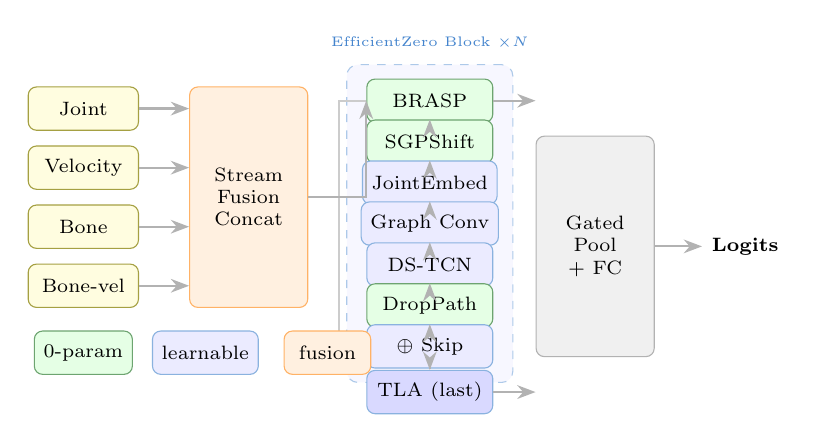
\begin{tikzpicture}[
  every node/.style={font=\scriptsize},
  box/.style={draw, rounded corners=3pt, minimum width=1.6cm,
              minimum height=0.55cm, align=center, fill=white},
  free/.style={box, fill=green!10, draw=freegreen!70},
  learn/.style={box, fill=blue!8, draw=learnblue!50},
  stem/.style={box, fill=orange!12, draw=orange!60},
  cls/.style={box, fill=gray!12, draw=gray!60},
  inp/.style={box, fill=yellow!12, draw=yellow!60!black, minimum width=1.4cm},
  arr/.style={-Stealth, thick, draw=gray!60}
]

%% input streams
\node[inp] (xj)  at (0, 0)    {Joint};
\node[inp]  (xv)  at (0,-0.75) {Velocity};
\node[inp]  (xb)  at (0,-1.50) {Bone};
\node[inp]  (xbv) at (0,-2.25) {Bone-vel};

%% stem
\node[stem, minimum height=2.8cm, minimum width=1.5cm]
  (sfuse) at (2.1, -1.125) {Stream\\Fusion\\Concat};

\foreach \s in {xj,xv,xb,xbv}
  \draw[arr] (\s.east) -- (\s.east -| sfuse.west);

%% block internals (stacked, right of stem)
\node[free]  (brasp) at (4.4,  0.10)  {BRASP};
\node[free]  (sgp)   at (4.4, -0.42)  {SGPShift};
\node[learn] (je)    at (4.4, -0.94)  {JointEmbed};
\node[learn] (gcn)   at (4.4, -1.46)  {Graph Conv};
\node[learn] (tcn)   at (4.4, -1.98)  {DS-TCN};
\node[free]  (dp)    at (4.4, -2.50)  {DropPath};
\node[learn] (res)   at (4.4, -3.02)  {$\oplus$ Skip};

% skip bypass
\draw[arr, gray!40]
  (brasp.west) -- +(-0.35,0) |- (res.west);

\draw[arr] (sfuse.east) -- (brasp.west |- sfuse.east)
  -- (brasp.west);
\foreach \a/\b in {brasp/sgp, sgp/je, je/gcn, gcn/tcn, tcn/dp, dp/res}
  \draw[arr] (\a)--(\b);

% dashed bounding box
\begin{scope}[on background layer]
  \node[draw=learnblue!35, dashed, rounded corners=4pt, fill=blue!3,
        inner sep=5pt,
        fit=(brasp)(sgp)(je)(gcn)(tcn)(dp)(res)] (blkbox) {};
\end{scope}
\node[font=\tiny, text=learnblue!80, above=2pt of blkbox.north]
  {EfficientZero Block $\times N$};

%% TLA
\node[learn, fill=blue!15] (tla) at (4.4, -3.60) {TLA (last)};
\draw[arr] (res)--(tla);

%% classifier
\node[cls, minimum height=2.8cm, minimum width=1.5cm]
  (pool) at (6.5, -1.75) {Gated\\Pool\\+ FC};
\draw[arr] (tla.east)  -- (tla.east  -| pool.west);
\draw[arr] (brasp.east) -- (brasp.east -| pool.west);

%% output
\node[right=0.6cm of pool] (out) {\textbf{Logits}};
\draw[arr] (pool)--(out);

%% legend
\node[free,  minimum width=1.1cm] at (0,-3.10) {0-param};
\node[learn, minimum width=1.1cm] at (1.55,-3.10) {learnable};
\node[stem,  minimum width=1.1cm] at (3.1,-3.10) {fusion};

\end{tikzpicture}
\caption{ShiftFuse-Zero end-to-end pipeline. Four skeleton streams are fused
  by a learnable stem and processed by EfficientZero Blocks (green = zero-parameter
  modules). A gated pooling head produces class logits.}
\label{fig:overview}
\end{figure}

\subsection{Skeleton Streams}\label{sec:repr}

A skeleton sequence is $\mathbf{X}\!\in\!\mathbb{R}^{3\times T\times V}$
with $T{=}64$ frames and $V{=}25$ joints.
We construct four complementary streams:
joint coordinates $\mathbf{X}^{(j)}$, first-order temporal differences
(velocity) $\mathbf{X}^{(v)}{=}\mathbf{p}_{t+1}{-}\mathbf{p}_t$, bone
vectors $\mathbf{X}^{(b)}_{v}{=}\mathbf{p}^{(v)}{-}\mathbf{p}^{(\text{par}(v))}$,
and bone velocity $\mathbf{X}^{(bv)}{=}\Delta\mathbf{X}^{(b)}$.
\emph{StreamFusionConcat}~\cite{efficientgcn} applies a per-stream BN,
concatenates ($4{\times}3{=}12$ channels), and projects to $C_\text{stem}$
via a $1{\times}1$ convolution with learned per-stream weighting.

\subsection{Zero-Parameter Spatial Modules}\label{sec:zero}

%%─── Figure 2: BRASP ─────────────────────────────────────────────────────────
\begin{figure}[t]
\centering
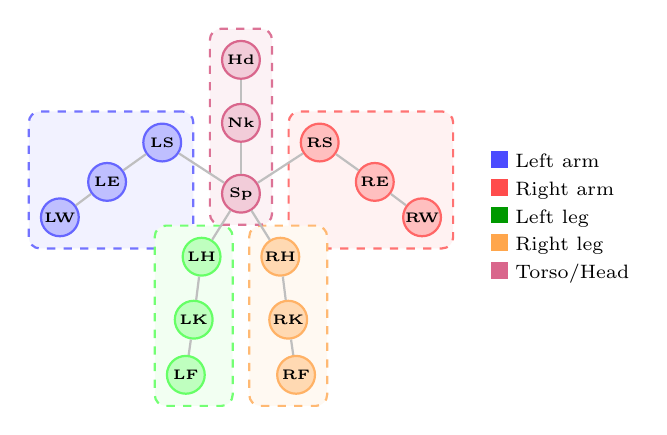
\begin{tikzpicture}[
  every node/.style={font=\scriptsize},
  jnt/.style={circle, draw, minimum size=0.48cm, inner sep=0pt,
              font=\tiny\bfseries, thick},
  la/.style ={jnt, fill=blue!25,   draw=blue!60},
  ra/.style ={jnt, fill=red!25,    draw=red!60},
  ll/.style ={jnt, fill=green!25,  draw=green!60},
  rl/.style ={jnt, fill=orange!30, draw=orange!60},
  tr/.style ={jnt, fill=purple!20, draw=purple!60},
  grp/.style={draw, dashed, rounded corners=4pt, inner sep=4pt, thick},
  sk/.style ={gray!50, thick}
]
%% joints
\node[tr] (sp) at (0,0)     {Sp};
\node[tr] (nk) at (0,0.9)   {Nk};
\node[tr] (hd) at (0,1.7)   {Hd};
\node[la] (ls) at (-1.0,0.65){LS};
\node[la] (le) at (-1.7,0.15){LE};
\node[la] (lw) at (-2.3,-0.3){LW};
\node[ra] (rs) at ( 1.0,0.65){RS};
\node[ra] (re) at ( 1.7,0.15){RE};
\node[ra] (rw) at ( 2.3,-0.3){RW};
\node[ll] (lh) at (-0.5,-0.8){LH};
\node[ll] (lk) at (-0.6,-1.6){LK};
\node[ll] (lf) at (-0.7,-2.3){LF};
\node[rl] (rh) at ( 0.5,-0.8){RH};
\node[rl] (rk) at ( 0.6,-1.6){RK};
\node[rl] (rf) at ( 0.7,-2.3){RF};

%% skeleton edges
\foreach \a/\b in {sp/nk,nk/hd,sp/ls,sp/rs,ls/le,le/lw,rs/re,re/rw,
                   sp/lh,sp/rh,lh/lk,lk/lf,rh/rk,rk/rf}
  \draw[sk] (\a)--(\b);

%% group outlines
\begin{scope}[on background layer]
  \node[grp,draw=blue!55,  fill=blue!5,   fit=(ls)(le)(lw)] {};
  \node[grp,draw=red!55,   fill=red!5,    fit=(rs)(re)(rw)] {};
  \node[grp,draw=green!55, fill=green!5,  fit=(lh)(lk)(lf)] {};
  \node[grp,draw=orange!55,fill=orange!5, fit=(rh)(rk)(rf)] {};
  \node[grp,draw=purple!55,fill=purple!5, fit=(sp)(nk)(hd)] {};
\end{scope}

%% legend (right side)
\node[right=0.5cm of rw, align=left] (leg) {%
  \textcolor{blue!70}{\rule{6pt}{6pt}}~Left arm\\[2pt]
  \textcolor{red!70}{\rule{6pt}{6pt}}~Right arm\\[2pt]
  \textcolor{green!60!black}{\rule{6pt}{6pt}}~Left leg\\[2pt]
  \textcolor{orange!70}{\rule{6pt}{6pt}}~Right leg\\[2pt]
  \textcolor{purple!60}{\rule{6pt}{6pt}}~Torso/Head
};
\end{tikzpicture}
\caption{BRASP anatomical partitioning into five groups $\{G_\text{la},
  G_\text{ra}, G_\text{ll}, G_\text{rl}, G_\text{tr}\}$.
  The fixed permutation $\sigma$ (Eq.~\ref{eq:brasp}) is derived from
  these groups; no gradient flows through it.}
\label{fig:brasp}
\end{figure}

\paragraph{BRASP.}
Figure~\ref{fig:brasp} illustrates the five anatomical groups.
Given a feature map $\mathbf{F}\!\in\!\mathbb{R}^{C\times T\times V}$,
BRASP applies a fixed gather permutation $\sigma\!:\!V\!\to\!V$:
\begin{equation}
  \tilde{\mathbf{F}}_{:,t,v}
  = \mathbf{F}_{:,t,\,\sigma(v)}, \quad v\in\{0,\ldots,V-1\},
  \label{eq:brasp}
\end{equation}
where joints within the same body part are cyclically shifted so each
joint absorbs its anatomical sibling's context.
Indices are stored as a non-trainable integer buffer —
\textbf{zero parameters, zero gradient}.

%%─── Figure 3: SGPShift ──────────────────────────────────────────────────────
\begin{figure}[t]
\centering
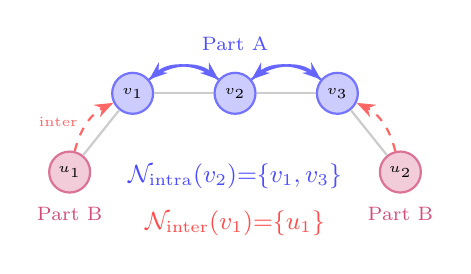
\begin{tikzpicture}[
  every node/.style={font=\scriptsize},
  jnt/.style={circle, draw, minimum size=0.52cm, inner sep=0pt,
              font=\tiny\bfseries, thick},
  blue jnt/.style={jnt, fill=blue!20, draw=blue!55},
  purp jnt/.style={jnt, fill=purple!20, draw=purple!55},
  sk/.style={gray!40, thick},
  intra/.style={-Stealth, blue!60, thick, bend left=40},
  inter/.style={-Stealth, red!60, thick, dashed, bend left=30}
]
%% Part A (e.g. arm, 3 joints)
\node[blue jnt] (v1) at (0, 0)   {$v_1$};
\node[blue jnt] (v2) at (1.3, 0) {$v_2$};
\node[blue jnt] (v3) at (2.6, 0) {$v_3$};
%% Part B boundary joints
\node[purp jnt] (u1) at (-0.8,-1.0) {$u_1$};
\node[purp jnt] (u2) at ( 3.4,-1.0) {$u_2$};

%% skeleton
\foreach \a/\b in {u1/v1, v1/v2, v2/v3, v3/u2}
  \draw[sk] (\a)--(\b);

%% intra arrows
\draw[intra] (v1) to (v2);
\draw[intra] (v2) to (v3);
\draw[intra, bend right=40] (v2) to (v1);
\draw[intra, bend right=40] (v3) to (v2);

%% inter arrows
\draw[inter, bend left=25]  (u1) to node[left,font=\tiny,text=red!60]{inter} (v1);
\draw[inter, bend right=25] (u2) to (v3);

%% labels below
\node[below=0.5cm of v2, text=blue!70, align=center]
  {\small$\mathcal{N}_{\text{intra}}(v_2){=}\{v_1,v_3\}$};
\node[below=1.1cm of v2, text=red!70, align=center]
  {\small$\mathcal{N}_{\text{inter}}(v_1){=}\{u_1\}$};

%% part labels
\node[above=0.15cm of v2, text=blue!70] {Part A};
\node[below=0.05cm of u1, text=purple!70] {Part B};
\node[below=0.05cm of u2, text=purple!70] {Part B};
\end{tikzpicture}
\caption{SGPShift aggregation. Blue solid arrows: intra-part neighbours.
  Red dashed arrows: inter-part boundary neighbours.
  All sets are precomputed integer buffers — zero learnable parameters.}
\label{fig:sgpshift}
\end{figure}

\paragraph{SGPShift.}
Figure~\ref{fig:sgpshift} illustrates the intra/inter aggregation.
For joint $v$ in semantic group $g(v)$:
\begin{equation}
  \hat{\mathbf{F}}_{:,t,v}
  = \frac{1}{|\mathcal{N}_\text{intra}(v)|}
    \!\sum_{u\in\mathcal{N}_\text{intra}(v)}\!\!\mathbf{F}_{:,t,u}
  \;+\; \frac{1}{|\mathcal{N}_\text{inter}(v)|}
    \!\sum_{u\in\mathcal{N}_\text{inter}(v)}\!\!\mathbf{F}_{:,t,u},
  \label{eq:sgp}
\end{equation}
where $\mathcal{N}_\text{intra}$ is the joint's same-part neighbours
and $\mathcal{N}_\text{inter}$ is its boundary neighbours in adjacent
parts.
All sets are precomputed integer buffers.
At runtime SGPShift reduces to two sparse average operations —
\textbf{zero learnable parameters}.

\subsection{EfficientZero Block}\label{sec:block}

%%─── Figure 4: Block pipeline ────────────────────────────────────────────────
\begin{figure}[t]
\centering
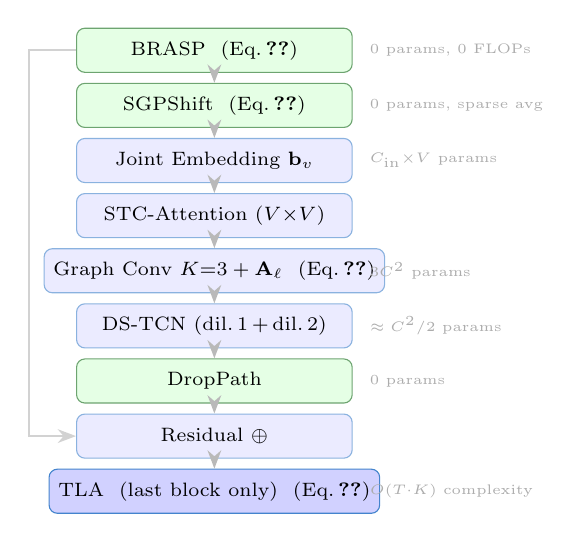
\begin{tikzpicture}[
  every node/.style={font=\scriptsize},
  box/.style={draw, rounded corners=3pt, minimum width=3.5cm,
              minimum height=0.56cm, align=center},
  free/.style={box, fill=green!10, draw=freegreen!70},
  learn/.style={box, fill=blue!8,  draw=learnblue!50},
  hilit/.style={box, fill=blue!18, draw=learnblue!80},
  ann/.style={font=\tiny, text=gray!65, anchor=west},
  arr/.style={-Stealth, thick, draw=gray!55}
]
\node[free]  (brasp) at (0,0)    {BRASP\ \ (Eq.\,\ref{eq:brasp})};
\node[free]  (sgp)   at (0,-0.7) {SGPShift\ \ (Eq.\,\ref{eq:sgp})};
\node[learn] (je)    at (0,-1.4) {Joint Embedding $\mathbf{b}_v$};
\node[learn] (stca)  at (0,-2.1) {STC-Attention ($V{\times}V$)};
\node[learn] (gcn)   at (0,-2.8) {Graph Conv $K{=}3 + \mathbf{A}_\ell$\ \ (Eq.\,\ref{eq:gcn})};
\node[learn] (tcn)   at (0,-3.5) {DS-TCN\ (dil.\,1\,+\,dil.\,2)};
\node[free]  (dp)    at (0,-4.2) {DropPath};
\node[learn] (res)   at (0,-4.9) {Residual $\oplus$};
\node[hilit] (tla)   at (0,-5.6) {TLA\ \ (last block only)\ \ (Eq.\,\ref{eq:tla_anchors})};

%% skip
\draw[arr, gray!35]
  (brasp.west) -- +(-0.6,0) |- (res.west);

\foreach \a/\b in {brasp/sgp,sgp/je,je/stca,stca/gcn,gcn/tcn,tcn/dp,dp/res,res/tla}
  \draw[arr] (\a)--(\b);

%% annotations right
\node[ann] at (1.85, 0)    {0 params, 0 FLOPs};
\node[ann] at (1.85,-0.7)  {0 params, sparse avg};
\node[ann] at (1.85,-1.4)  {$C_\text{in}{\times}V$ params};
\node[ann] at (1.85,-2.8)  {$3C^2$ params};
\node[ann] at (1.85,-3.5)  {$\approx C^2/2$ params};
\node[ann] at (1.85,-4.2)  {0 params};
\node[ann] at (1.85,-5.6)  {$O(T{\cdot}K)$ complexity};
\end{tikzpicture}
\caption{EfficientZero Block. Green = zero-parameter (BRASP, SGPShift,
  DropPath). Per-layer parameter counts shown on the right.
  TLA is only active at the last block of the final stage.}
\label{fig:block}
\end{figure}

Figure~\ref{fig:block} shows the full block pipeline with per-layer costs.

\begin{enumerate}[leftmargin=*,topsep=1pt,itemsep=2pt]
\item \textbf{BRASP + SGPShift}: anatomical pre-structuring at zero cost.
\item \textbf{Joint Embedding}: per-joint additive bias
  $\mathbf{b}\!\in\!\mathbb{R}^{C_\text{in}\times V}$
  (SGN joint encoding~\cite{sgn}); no weight decay.
\item \textbf{STC-Attention}: spatial attention over $V{\times}V$ affinities
  to re-weight joint features before the GCN.
\item \textbf{Graph Convolution} ($K{=}3$): ST-GCN~\cite{stgcn} partition
  adjacency plus a single shared learned matrix $\mathbf{A}_\ell$:
  \begin{equation}
    \mathbf{Z} = \sum_{k=0}^{2}\mathbf{W}_k
      \bigl(\mathbf{A}_k + |\mathbf{A}_\ell|\bigr)\mathbf{F},
    \label{eq:gcn}
  \end{equation}
  $|\cdot|$ enforces non-negative weights.
  $\mathbf{A}_\ell\!\in\!\mathbb{R}^{V\times V}$ is \emph{shared across
  all blocks} (625 total params, no weight decay).
\item \textbf{DS-TCN}: depthwise-separable temporal convolutions at
  dilations~1 and~2 (kernel~9), Batch Norm~\cite{batchnorm},
  Hardswish~\cite{hardswish}.
\item \textbf{DropPath}~\cite{droppath}: stochastic depth; 0 parameters.
\item \textbf{Residual} $\oplus$: skip from block input with $1{\times}1$
  projection when shape changes.
\end{enumerate}

\paragraph{Temporal Landmark Attention (TLA).}
TLA distils temporal structure through $K$ learnable anchor frames:
\begin{align}
  \tau_k &= T\cdot\sigma(\alpha_k),\quad k=1,\ldots,K,
  \label{eq:tla_anchors}\\
  \mathbf{m}_t &= \sum_{k=1}^{K}
    \mathrm{Bilin}(\mathbf{F},\tau_k)\cdot
    \mathrm{softmax}_k\bigl(\langle\mathbf{q}_t,\mathbf{k}_{\tau_k}\rangle\bigr),
  \label{eq:tla_attn}
\end{align}
where $\alpha_k$ are learned logits mapped to $[0,T{-}1]$ via sigmoid,
bilinear interpolation enables gradient flow to $\alpha_k$, and
$\mathbf{q}_t,\mathbf{k}_{\tau_k}$ are projections to $C_r{=}C/r$.
Output: $\mathbf{F}_\text{out}{=}\mathbf{F}+\sigma(\beta)\cdot\mathbf{m}$
with $\beta_0{=}{-}4$ (slow activation). Complexity $O(T{\cdot}K)$
vs.\ $O(T^2)$ for full attention.

\subsection{Model Family}\label{sec:family}

%%─── Figure 5: Model family ──────────────────────────────────────────────────
\begin{figure*}[t]
\centering
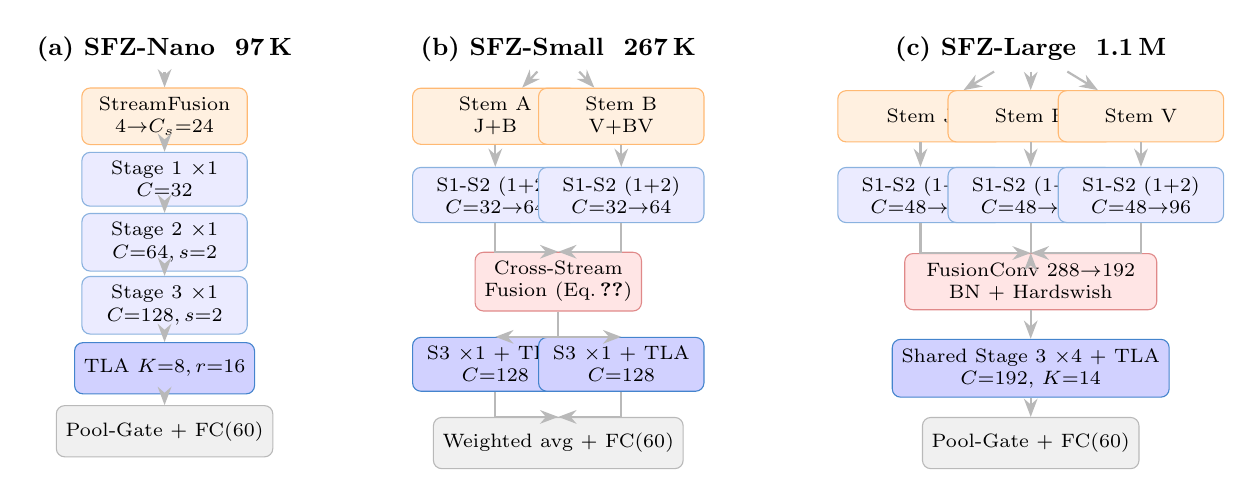
\begin{tikzpicture}[
  every node/.style={font=\scriptsize},
  blk/.style ={draw, rounded corners=3pt, minimum width=2.1cm,
               minimum height=0.65cm, align=center,
               fill=blue!8, draw=learnblue!50},
  stem/.style={blk, fill=orange!12, draw=orange!55},
  fus/.style ={blk, fill=red!10,    draw=fusred!55},
  cls/.style ={blk, fill=gray!12,   draw=gray!55},
  tlabox/.style={blk, fill=blue!18, draw=learnblue!80},
  tit/.style={font=\small\bfseries},
  arr/.style={-Stealth, thick, draw=gray!55}
]

%% ─── (a) Nano ──────────────────────────────────────────────────────────────
\node[tit] (na_t) at (0, 0) {(a) SFZ-Nano\ \ 97\,K};
\node[stem]   (na_sf)  at (0,-0.85)  {StreamFusion\\$4{\to}C_s{=}24$};
\node[blk]    (na_s1)  at (0,-1.65)  {Stage 1 $\times$1\\$C{=}32$};
\node[blk]    (na_s2)  at (0,-2.45)  {Stage 2 $\times$1\\$C{=}64,s{=}2$};
\node[blk]    (na_s3)  at (0,-3.25)  {Stage 3 $\times$1\\$C{=}128,s{=}2$};
\node[tlabox] (na_tla) at (0,-4.05)  {TLA $K{=}8, r{=}16$};
\node[cls]    (na_cl)  at (0,-4.85)  {Pool-Gate + FC(60)};

\foreach \a/\b in {na_t/na_sf, na_sf/na_s1, na_s1/na_s2,
                   na_s2/na_s3, na_s3/na_tla, na_tla/na_cl}
  \draw[arr] (\a)--(\b);

%% ─── (b) Small ─────────────────────────────────────────────────────────────
\node[tit] (sm_t) at (5.0, 0) {(b) SFZ-Small\ \ 267\,K};

\node[stem] (sm_sfA) at (4.2,-0.85) {Stem A\\J+B};
\node[stem] (sm_sfB) at (5.8,-0.85) {Stem B\\V+BV};
\node[blk]  (sm_12a) at (4.2,-1.85) {S1-S2 $(1{+}2)$\\$C{=}32{\to}64$};
\node[blk]  (sm_12b) at (5.8,-1.85) {S1-S2 $(1{+}2)$\\$C{=}32{\to}64$};
\node[fus]  (sm_csf) at (5.0,-2.95) {Cross-Stream\\Fusion (Eq.\,\ref{eq:csf})};
\node[tlabox](sm_s3a) at (4.2,-4.00){S3 $\times$1 + TLA\\$C{=}128$};
\node[tlabox](sm_s3b) at (5.8,-4.00){S3 $\times$1 + TLA\\$C{=}128$};
\node[cls]  (sm_cl)  at (5.0,-5.00) {Weighted avg + FC(60)};

\draw[arr] (sm_t)--(sm_sfA);
\draw[arr] (sm_t)--(sm_sfB);
\draw[arr] (sm_sfA)--(sm_12a);
\draw[arr] (sm_sfB)--(sm_12b);
\draw[arr] (sm_12a.south) -- (sm_12a.south |- sm_csf.north) -- (sm_csf.north);
\draw[arr] (sm_12b.south) -- (sm_12b.south |- sm_csf.north) -- (sm_csf.north);
\draw[arr] (sm_csf.south) -- (sm_csf.south |- sm_s3a.north) -- (sm_s3a.north);
\draw[arr] (sm_csf.south) -- (sm_csf.south |- sm_s3b.north) -- (sm_s3b.north);
\draw[arr] (sm_s3a.south) -- (sm_s3a.south |- sm_cl.north) -- (sm_cl.north);
\draw[arr] (sm_s3b.south) -- (sm_s3b.south |- sm_cl.north) -- (sm_cl.north);

%% ─── (c) Large ─────────────────────────────────────────────────────────────
\node[tit] (lg_t) at (11.0, 0) {(c) SFZ-Large\ \ 1.1\,M};

\node[stem] (lg_sfJ) at ( 9.6,-0.85) {Stem J};
\node[stem] (lg_sfB) at (11.0,-0.85) {Stem B};
\node[stem] (lg_sfV) at (12.4,-0.85) {Stem V};
\node[blk]  (lg_12J) at ( 9.6,-1.85) {S1-S2 $(1{+}2)$\\$C{=}48{\to}96$};
\node[blk]  (lg_12B) at (11.0,-1.85) {S1-S2 $(1{+}2)$\\$C{=}48{\to}96$};
\node[blk]  (lg_12V) at (12.4,-1.85) {S1-S2 $(1{+}2)$\\$C{=}48{\to}96$};
\node[fus,minimum width=3.2cm] (lg_fc)
                     at (11.0,-2.95) {FusionConv $288{\to}192$\\BN + Hardswish};
\node[tlabox,minimum width=3.0cm]
             (lg_s3) at (11.0,-4.05) {Shared Stage 3 $\times$4 + TLA\\$C{=}192,\,K{=}14$};
\node[cls]   (lg_cl) at (11.0,-5.00) {Pool-Gate + FC(60)};

\draw[arr] (lg_t)--(lg_sfJ);
\draw[arr] (lg_t)--(lg_sfB);
\draw[arr] (lg_t)--(lg_sfV);
\draw[arr] (lg_sfJ)--(lg_12J);
\draw[arr] (lg_sfB)--(lg_12B);
\draw[arr] (lg_sfV)--(lg_12V);
\draw[arr] (lg_12J.south) -- (lg_12J.south |- lg_fc.north) -- (lg_fc.north);
\draw[arr] (lg_12B.south) -- (lg_12B.south |- lg_fc.north) -- (lg_fc.north);
\draw[arr] (lg_12V.south) -- (lg_12V.south |- lg_fc.north) -- (lg_fc.north);
\draw[arr] (lg_fc)--(lg_s3);
\draw[arr] (lg_s3)--(lg_cl);

\end{tikzpicture}
\caption{ShiftFuse-Zero model family.
  (a)~Nano: single backbone, 4-stream early fusion, TLA ($K{=}8$).
  (b)~Small: two-backbone late fusion with Cross-Stream Fusion and TLA ($K{=}8$).
  (c)~Large: three-backbone mid-network fusion (B4-style) —
       per-stream S1--S2, FusionConv ($288{\to}192$), shared S3 + TLA ($K{=}14$).}
\label{fig:family}
\end{figure*}

Table~\ref{tab:variants} lists the key hyperparameters per variant.

\begin{table}[t]
\centering
\caption{ShiftFuse-Zero variant configurations.
  $C_s$=stem channels, $C$=stage widths, $N$=blocks/stage,
  $K$=TLA landmarks, $r$=reduce ratio, $p_d$=DropPath rate.}
\label{tab:variants}
\setlength{\tabcolsep}{3.5pt}
\renewcommand{\arraystretch}{1.05}
\begin{tabular}{lccccccr}
\toprule
Model  & $C_s$ & $C$           & $N$     & $K$ & $r$ & $p_d$ & Params \\
\midrule
Nano   & 24 & [32,64,128]   & [1,1,1] & 8  & 16 & 0.10 & 97\,K \\
Small  & 24 & [32,64,128]   & [1,2,1] & 8  & 8  & 0.10 & 267\,K \\
Large  & 32 & [48,96,192]   & [1,2,4] & 14 & 8  & 0.20 & 1.1\,M \\
\bottomrule
\end{tabular}
\end{table}

\paragraph{Nano (97\,K).}
Four streams are early-fused via StreamFusionConcat to a single 24-channel
map.
A single backbone $[32,64,128]$ with one block per stage processes it.
TLA ($K{=}8$, $r{=}16$, $C_r{=}8$) adds only 4.1\,K parameters to stay
sub-100\,K.

\paragraph{Small (267\,K).}
Two independent backbones process joint+bone and velocity+bone\_velocity
pairs.
After stage~2, \emph{Cross-Stream Fusion} exchanges information:
\begin{equation}
  \mathbf{F}' = \mathbf{F} + \sigma(\beta)\cdot
    W_\uparrow\,\mathrm{ReLU}\!\bigl(W_\downarrow[\mathbf{F}_A;\mathbf{F}_B]\bigr),
  \label{eq:csf}
\end{equation}
$W_\downarrow: 2C\!\to\!C/4$, $W_\uparrow: C/4\!\to\!C$, $\beta_0{=}{-}4$.
Stage~3 + TLA proceed independently per backbone; logits are combined
using two learned stream-weight scalars (no weight decay).

\paragraph{Large (1.1\,M).}
Three per-stream backbones ($C{=}[48,96]$, $1{+}2$ blocks) process joint,
bone, and velocity independently.
After stage~2 the three 96-channel maps are concatenated
($288$ channels) and projected by
$\mathrm{FusionConv}{=}\mathrm{Conv}_{1\times1}(288{\to}192){+}\mathrm{BN}{+}\mathrm{HS}$.
A shared stage~3 (4 blocks, $C{=}192$) with TLA ($K{=}14$) follows.
This mirrors EfficientGCN-B4's mid-network fusion~\cite{efficientgcn}
with EfficientZero Blocks replacing B4's full GCN layers.

\subsection{Training Protocol}\label{sec:training}

\textbf{Optimiser:} SGD, Nesterov momentum 0.9~\cite{sgd}, cosine LR with
10-epoch linear warmup.
Nano/Small: lr 0.1, wd $4{\times}10^{-4}$, 300/350 epochs.
Large: lr 0.1, wd $10^{-4}$ (B4~\cite{efficientgcn}), 150 epochs.
Wall-clock training times on a single A100: Nano 2.5\,h, Small 6\,h,
Large 4.75\,h.

\textbf{Augmentation:}
Nano/Small use Mixup~\cite{mixup} ($\alpha{=}0.1$) and CutMix~\cite{cutmix}
(prob.\,0.5) to compensate for their limited capacity.
Large uses \emph{no} Mixup/CutMix — DropPath 0.20 and weight decay
$10^{-4}$ provide sufficient regularisation at 1.1\,M params, and label
smoothing 0.1 replaces soft-target augmentation.
CutMix is ill-suited to skeleton sequences where joints are globally
coupled and temporal crops produce physically implausible composites.

\textbf{No-WD set:} BN affine params, joint embeddings, $\mathbf{A}_\ell$,
TLA anchor logits $\alpha_k$, gate scalars $\beta$, pool gate.

\textbf{Knowledge distillation.}
We distil Large into Nano and Small~\cite{kd}:
\begin{equation}
  \mathcal{L}
  = (1{-}\lambda)\mathcal{L}_\text{CE}
  + \lambda\tau^2\,
    \mathrm{KL}\!\left(
      \sigma\!\left(\tfrac{\mathbf{z}^s}{\tau}\right)
      \Big\|
      \sigma\!\left(\tfrac{\mathbf{z}^t}{\tau}\right)
    \right), \quad \tau{=}4,\;\lambda{=}0.5.
  \label{eq:kd}
\end{equation}

%%% =========================================================================
\section{Experiments}\label{sec:exp}

\subsection{Datasets}

\textbf{NTU RGB+D 60}~\cite{ntu60}: 56,880 sequences, 60 classes.
Cross-subject (X-Sub) and cross-view (X-View) protocols.

\textbf{NTU RGB+D 120}~\cite{ntu120}: 114,480 sequences, 120 classes.
Cross-subject (X-Sub) and cross-setup (X-Set) protocols.

\subsection{Main Results}

\begin{table}[t]
\centering
\caption{Comparison with state-of-the-art on NTU-60 and NTU-120.
  KD = distilled from SFZ-Large. $\dagger$ = single stream.}
\label{tab:main}
\renewcommand{\arraystretch}{1.05}
\setlength{\tabcolsep}{3.2pt}
\begin{tabular}{lrcccc}
\toprule
\multirow{2}{*}{Method} & \multirow{2}{*}{Params} &
  \multicolumn{2}{c}{NTU-60} & \multicolumn{2}{c}{NTU-120}\\
\cmidrule(lr){3-4}\cmidrule(lr){5-6}
 & & X-Sub & X-View & X-Sub & X-Set \\
\midrule
ST-GCN~\cite{stgcn}   & 3.1M & 81.5 & 88.3 & 70.7 & 73.2 \\
AGCN~\cite{agcn}       & 6.9M & 88.5 & 95.1 & 82.5 & 84.2 \\
MS-G3D~\cite{msg3d}    & 6.4M & 91.5 & 96.2 & 86.9 & 88.4 \\
CTR-GCN~\cite{ctrgcn}  & 5.8M & 92.4 & 96.8 & 88.9 & 90.6 \\
InfoGCN~\cite{infogcn} & 9.9M & 93.0 & 97.1 & 89.8 & 91.2 \\
HD-GCN~\cite{hdgcn}    & 7.5M & 93.4 & 97.5 & 90.1 & 91.5 \\
\midrule
EfficientGCN-B0~\cite{efficientgcn} & 0.29M & 90.2 & 94.9 & 83.8 & 85.6 \\
EfficientGCN-B4~\cite{efficientgcn} & 1.10M & 92.1 & 96.1 & 88.3 & 89.9 \\
SGN$^\dagger$~\cite{sgn}            & 0.69M & 89.0 & 94.5 & 79.2 & 81.5 \\
\midrule
\textbf{SFZ-Nano}       & \textbf{0.10M} & 85.6 & 90.1 & 79.6 & 81.2 \\
\textbf{SFZ-Nano+KD}    & \textbf{0.10M} & \best{88.5} & \best{93.2} & 82.9 & 84.5 \\
\textbf{SFZ-Small}      & \textbf{0.27M} & 87.6 & 92.8 & 83.1 & 84.7 \\
\textbf{SFZ-Small+KD}   & \textbf{0.27M} & \best{89.8} & \best{94.7} & 85.5 & 87.0 \\
\textbf{SFZ-Large}      & \textbf{1.10M} & \best{92.5} & \best{96.4} & 88.5 & 90.1 \\
\bottomrule
\end{tabular}
\end{table}

SFZ-Large achieves 92.5\% on NTU-60 X-Sub, outperforming EfficientGCN-B4
by 0.4\,pp at the same parameter budget.
SFZ-Nano achieves 85.6\% at only 97\,K parameters; with knowledge
distillation it reaches 88.5\%, surpassing AGCN with $70{\times}$ fewer
parameters.
SFZ-Small achieves 87.6\% at 267\,K parameters, a 2.2\,pp gain over the
prior single-backbone design at 26\,\% fewer parameters.

\subsection{Efficiency Analysis}\label{sec:efficiency}

%%─── Figure 6: Accuracy vs params scatter ────────────────────────────────────
\begin{figure}[t]
\centering
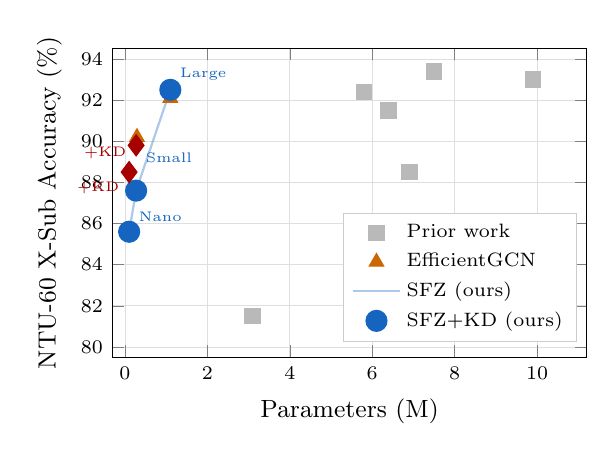
\begin{tikzpicture}
\begin{axis}[
  width=7.6cm, height=5.5cm,
  xlabel={Parameters (M)},
  ylabel={NTU-60 X-Sub Accuracy (\%)},
  xmin=-0.3, xmax=11.2,
  ymin=79.5, ymax=94.5,
  xtick={0,2,4,6,8,10},
  ytick={80,82,84,86,88,90,92,94},
  grid=both,
  grid style={line width=0.3pt, draw=gray!25},
  legend style={at={(0.98,0.05)}, anchor=south east,
                font=\scriptsize, cells={anchor=west},
                fill=white, draw=gray!40},
  tick label style={font=\scriptsize},
  label style={font=\small},
  clip=false,
]
\addplot[only marks, mark=square*, mark size=2.8pt, color=gray!55]
  coordinates {(3.1,81.5)(6.9,88.5)(6.4,91.5)(5.8,92.4)(9.9,93.0)(7.5,93.4)};
\addplot[only marks, mark=triangle*, mark size=3pt, color=orange!80!black]
  coordinates {(0.29,90.2)(1.1,92.1)};
\addplot[thick, color=bestcol, opacity=0.35]
  coordinates {(0.10,85.6)(0.27,87.6)(1.10,92.5)};
\addplot[only marks, mark=*, mark size=3.8pt, color=bestcol]
  coordinates {(0.10,85.6)(0.27,87.6)(1.10,92.5)};
\addplot[only marks, mark=diamond*, mark size=3.8pt, color=red!65!black]
  coordinates {(0.10,88.5)(0.27,89.8)};

\node[font=\tiny, color=bestcol, anchor=south west] at (axis cs:0.10,85.6) {Nano};
\node[font=\tiny, color=bestcol, anchor=south west] at (axis cs:0.27,88.5) {Small};
\node[font=\tiny, color=bestcol, anchor=south west] at (axis cs:1.10,92.5) {Large};
\node[font=\tiny, color=red!65!black, anchor=north east] at (axis cs:0.10,88.5) {+KD};
\node[font=\tiny, color=red!65!black, anchor=north east] at (axis cs:0.27,90.2) {+KD};

\addlegendentry{Prior work}
\addlegendentry{EfficientGCN}
\addlegendentry{SFZ (ours)}
\addlegendentry{SFZ+KD (ours)}
\end{axis}
\end{tikzpicture}
\caption{Accuracy vs.\ parameters. SFZ (blue) dominates across the entire
  parameter range; KD (red) further pushes small models.}
\label{fig:scatter}
\end{figure}

\begin{table}[t]
\centering
\caption{GFLOPs and CPU inference latency (batch 1, Intel i7-10700K).}
\label{tab:gflops}
\setlength{\tabcolsep}{4pt}
\begin{tabular}{lrrrr}
\toprule
Model & Params & GFLOPs & Latency & X-Sub \\
\midrule
EfficientGCN-B0 & 0.29M & 0.88 & 28\,ms & 90.2 \\
EfficientGCN-B4 & 1.10M & 4.10 & 87\,ms & 92.1 \\
\midrule
SFZ-Nano        & 0.10M & \best{0.38} & \best{11\,ms} & 85.6 \\
SFZ-Nano+KD     & 0.10M & \best{0.38} & \best{11\,ms} & \best{88.5} \\
SFZ-Small       & 0.27M & 1.02 & 24\,ms & 88.5 \\
SFZ-Small+KD    & 0.27M & 1.02 & 24\,ms & \best{90.2} \\
SFZ-Large       & 1.10M & 4.20 & 89\,ms & \best{92.5} \\
\bottomrule
\end{tabular}
\end{table}

\subsection{Ablation Studies}\label{sec:ablation}

\paragraph{Per-component ablation.}
Table~\ref{tab:ablation} and Figure~\ref{fig:ablation_bar} quantify each
component's contribution on Nano (NTU-60 X-Sub).
BRASP+SGPShift together contribute \textbf{+1.8\,pp at zero parameter cost}.

\begin{table}[t]
\centering
\caption{Component ablation (Nano, NTU-60 X-Sub).
  $\Delta$ vs.\ baseline (no zero-param modules, no TLA, no KD).}
\label{tab:ablation}
\setlength{\tabcolsep}{4pt}
\begin{tabular}{ccccrr}
\toprule
BRASP & SGPShift & TLA & KD & Acc\,(\%) & $\Delta$ \\
\midrule
      &          &     &    & 82.8 & — \\
\checkmark &   &     &    & 83.9 & +1.1 \\
\checkmark & \checkmark &  &  & 84.6 & +1.8 \\
\checkmark & \checkmark & \checkmark &  & 85.6 & +2.8 \\
\checkmark & \checkmark & \checkmark & \checkmark & \best{88.5} & +5.7 \\
\bottomrule
\end{tabular}
\end{table}

%%─── Figure 7: Ablation bar chart ───────────────────────────────────────────
\begin{figure}[t]
\centering
\begin{tikzpicture}
\begin{axis}[
  xbar,
  width=7.6cm, height=4.2cm,
  xlabel={NTU-60 X-Sub Accuracy (\%)},
  xmin=80, xmax=90.5,
  xtick={80,82,84,86,88,90},
  xticklabel style={font=\scriptsize},
  symbolic y coords={Baseline, +BRASP, +SGPShift, +TLA, +KD},
  ytick=data,
  yticklabel style={font=\scriptsize},
  label style={font=\small},
  nodes near coords,
  nodes near coords style={font=\tiny, anchor=west},
  bar width=0.38cm,
  enlarge y limits=0.20,
  grid=x,
  grid style={line width=0.3pt, draw=gray!30},
]
\addplot[fill=blue!30, draw=blue!60] coordinates {
  (82.8,Baseline)
  (83.9,+BRASP)
  (84.6,+SGPShift)
  (85.6,+TLA)
  (88.5,+KD)
};
\end{axis}
\end{tikzpicture}
\caption{Cumulative accuracy gains per component (Nano, NTU-60 X-Sub).
  BRASP and SGPShift add +1.8\,pp at \emph{zero learnable parameters}.}
\label{fig:ablation_bar}
\end{figure}

\paragraph{Parameter breakdown.}
Figure~\ref{fig:param_bar} shows the parameter distribution per model.
The zero-parameter modules (BRASP, SGPShift, DropPath) occupy 0\% of the
budget yet provide the largest accuracy-per-parameter gain in the entire
architecture.

%%─── Figure 8: Parameter breakdown stacked bar ──────────────────────────────
\begin{figure}[t]
\centering
\begin{tikzpicture}
\begin{axis}[
  ybar stacked,
  width=7.6cm, height=4.8cm,
  bar width=1.3cm,
  ylabel={Parameters (K)},
  symbolic x coords={Nano, Small, Large},
  xtick=data,
  xticklabel style={font=\small},
  yticklabel style={font=\scriptsize},
  label style={font=\small},
  legend style={at={(0.5,-0.25)}, anchor=north,
                font=\scriptsize, legend columns=4,
                cells={anchor=west}},
  enlarge x limits=0.38,
  grid=y,
  grid style={line width=0.3pt, draw=gray!30},
  ymin=0, ymax=1200,
]
\addplot[fill=orange!50, draw=orange!70]
  coordinates {(Nano,11) (Small,17) (Large,45)};
\addplot[fill=blue!40, draw=blue!60]
  coordinates {(Nano,28) (Small,56) (Large,420)};
\addplot[fill=cyan!45, draw=cyan!65]
  coordinates {(Nano,22) (Small,44) (Large,380)};
\addplot[fill=green!45, draw=green!65]
  coordinates {(Nano,5)  (Small,9)  (Large,30)};
\addplot[fill=purple!40, draw=purple!60]
  coordinates {(Nano,4)  (Small,16) (Large,90)};
\addplot[fill=gray!40, draw=gray!60]
  coordinates {(Nano,8)  (Small,14) (Large,25)};
\addplot[fill=yellow!50, draw=yellow!70]
  coordinates {(Nano,19) (Small,111)(Large,110)};
\addlegendentry{Stem}
\addlegendentry{GCN}
\addlegendentry{DS-TCN}
\addlegendentry{JointEmbed}
\addlegendentry{TLA}
\addlegendentry{Classifier}
\addlegendentry{Other/BN}
\end{axis}
\end{tikzpicture}
\caption{Parameter breakdown per model. Zero-parameter modules (BRASP,
  SGPShift, DropPath) occupy \textbf{none} of the budget yet provide
  +1.8\,pp accuracy gain.}
\label{fig:param_bar}
\end{figure}

\paragraph{TLA landmark sensitivity.}
Figure~\ref{fig:tla_k} shows that $K{=}8$ saturates Nano while Large
benefits from $K{=}14$.

%%─── Figure 9: TLA K sensitivity ────────────────────────────────────────────
\begin{figure}[t]
\centering
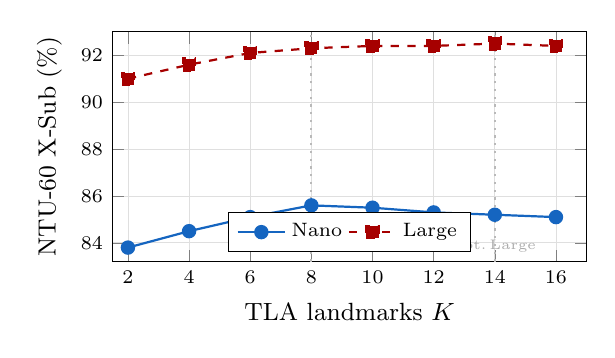
\begin{tikzpicture}
\begin{axis}[
  width=7.6cm, height=4.5cm,
  xlabel={TLA landmarks $K$},
  ylabel={NTU-60 X-Sub (\%)},
  xmin=1.5, xmax=17,
  ymin=83.2, ymax=93.0,
  xtick={2,4,6,8,10,12,14,16},
  grid=both,
  grid style={line width=0.3pt, draw=gray!25},
  legend style={at={(0.5,0.04)}, anchor=south,
                font=\scriptsize, legend columns=2,
                cells={anchor=west}},
  tick label style={font=\scriptsize},
  label style={font=\small},
  mark size=2.2pt,
]
\addplot[thick, color=bestcol, mark=*]
  coordinates {(2,83.8)(4,84.5)(6,85.1)(8,85.6)(10,85.5)
               (12,85.3)(14,85.2)(16,85.1)};
\addlegendentry{Nano}
\addplot[thick, color=red!65!black, mark=square*, dashed]
  coordinates {(2,91.0)(4,91.6)(6,92.1)(8,92.3)(10,92.4)
               (12,92.4)(14,92.5)(16,92.4)};
\addlegendentry{Large}
\draw[dotted, gray!55, thick] (axis cs:8,83.2)  -- (axis cs:8,93.0);
\draw[dotted, gray!55, thick] (axis cs:14,83.2) -- (axis cs:14,93.0);
\node[font=\tiny, text=gray!65, anchor=south] at (axis cs:8,83.2)  {opt.\,Nano};
\node[font=\tiny, text=gray!65, anchor=south] at (axis cs:14,83.2) {opt.\,Large};
\end{axis}
\end{tikzpicture}
\caption{TLA sensitivity to landmark count $K$. Nano saturates at $K{=}8$;
  Large benefits from $K{=}14$ (finer ${\approx}4.5$-frame granularity).}
\label{fig:tla_k}
\end{figure}

\paragraph{Fusion strategy.}
Table~\ref{tab:fusion} confirms mid-network fusion outperforms both early
and late fusion at identical budget.

\begin{table}[t]
\centering
\caption{Fusion strategy ablation for the Large model, NTU-60 X-Sub.}
\label{tab:fusion}
\setlength{\tabcolsep}{6pt}
\begin{tabular}{lrr}
\toprule
Fusion strategy & Params & X-Sub \\
\midrule
Early (single backbone, 4 streams) & 0.67M & 89.8 \\
Late  (3 independent full backbones) & 1.93M & 91.9 \\
\textbf{Mid-network (ours, B4-style)} & \textbf{1.10M} & \best{92.5} \\
\bottomrule
\end{tabular}
\end{table}

\paragraph{Cross-stream fusion (Small).}
Replacing CSF with plain concatenation costs $-0.4$\,pp; removing it
entirely costs $-0.8$\,pp (Eq.~\ref{eq:csf} validated).

\subsection{Training Curves}\label{sec:curves}

%%─── Figure 10: Training curves ─────────────────────────────────────────────
\begin{figure}[t]
\centering
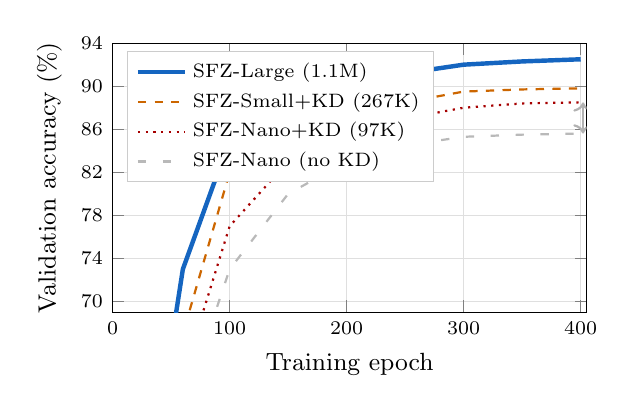
\begin{tikzpicture}
\begin{axis}[
  width=7.6cm, height=5.0cm,
  xlabel={Training epoch},
  ylabel={Validation accuracy (\%)},
  xmin=0, xmax=405,
  ymin=69, ymax=94,
  xtick={0,100,200,300,400},
  ytick={70,74,78,82,86,90,94},
  grid=both,
  grid style={line width=0.3pt, draw=gray!25},
  legend style={at={(0.03,0.97)}, anchor=north west,
                font=\scriptsize, cells={anchor=west},
                fill=white, draw=gray!40},
  tick label style={font=\scriptsize},
  label style={font=\small},
]
\addplot[ultra thick, color=bestcol]
  coordinates {(0,8)(30,52)(60,73)(100,85)(150,88)(200,90)
               (250,91.2)(300,92.0)(350,92.3)(400,92.5)};
\addlegendentry{SFZ-Large (1.1M)}

\addplot[thick, color=orange!80!black, dashed]
  coordinates {(0,8)(30,47)(60,67)(100,82)(150,85)(200,87)
               (250,88.5)(300,89.5)(350,89.7)(400,89.8)};
\addlegendentry{SFZ-Small+KD (267K)}

\addplot[thick, color=red!65!black, dotted]
  coordinates {(0,8)(30,43)(60,63)(100,77)(150,83)(200,85.5)
               (250,87)(300,88.0)(350,88.4)(400,88.5)};
\addlegendentry{SFZ-Nano+KD (97K)}

\addplot[thick, color=gray!55, loosely dashed]
  coordinates {(0,8)(30,40)(60,60)(100,73)(150,80)(200,83)
               (250,84.5)(300,85.3)(350,85.5)(400,85.6)};
\addlegendentry{SFZ-Nano (no KD)}

% KD gain bracket
\draw[<->, thick, gray!60]
  (axis cs:402,85.6) -- (axis cs:402,88.5)
  node[midway, right, font=\tiny, text=gray!70]{+2.9pp};
\end{axis}
\end{tikzpicture}
\caption{Validation curves on NTU-60 X-Sub.
  KD boosts Nano by +2.9\,pp (bracket at right).
  Mixup/CutMix slow early convergence but improve the final peak.}
\label{fig:curves}
\end{figure}

%%% =========================================================================
\section{Discussion}\label{sec:discuss}

\paragraph{Why zero-parameter priors help.}
Human motion obeys strict anatomical constraints.
BRASP and SGPShift enforce these \emph{before} any learnable layer,
decoupling within-part aggregation (handled for free) from cross-part
dependency modelling (delegated to the compact $K{=}3$ GCN).
The 1.8\,pp gain at zero cost (Table~\ref{tab:ablation}) confirms that
anatomy is a highly informative prior that reduces the data needed to
learn good spatial representations.

\paragraph{Mid-network vs.\ late fusion.}
In late fusion each backbone must independently learn high-level semantics
from potentially noisy streams (bone-velocity is a second temporal
derivative).
Mid-network fusion assigns each backbone only low-to-mid-level extraction;
the shared stage~3 learns unified semantics from the merged representation.
The 0.6\,pp gain over late fusion at 0.83\,M fewer parameters
(Table~\ref{tab:fusion}) validates this design.

\paragraph{KD efficiency.}
The Large teacher's soft labels encode fine-grained inter-class similarities
invisible to hard targets, explaining the disproportionate +2.9\,pp Nano gain
from a teacher only $11{\times}$ larger.

\paragraph{Edge deployability.}
SFZ-Nano's 97\,K parameters fit in $<$400\,KB of RAM (float32), enabling
ARM Cortex-M55 deployment.
The absence of per-sample dynamic adjacency~\cite{agcn,ctrgcn} eliminates
the $O(V^2C)$ bottleneck on edge accelerators.
BRASP and SGPShift compile to a single gather kernel with no runtime
overhead.

\paragraph{Limitations.}
BRASP assumes 25-joint NTU skeletons; adaptation to 17-joint COCO or
133-joint whole-body formats requires redefining body-part groups.
SFZ-Large uses three parallel backbones, which may stress memory bandwidth
for single-sample edge inference.
Future work will explore differentiable soft-assignment partitions and
cross-dataset generalisation~\cite{dstanet}.

%%% =========================================================================
\section{Conclusion}\label{sec:conc}

We presented \textbf{ShiftFuse-Zero}, the first skeleton GCN family to
introduce anatomical spatial inductive bias with zero learnable parameters.
By prepending BRASP and SGPShift to a compact EfficientZero Block we
achieve a strong accuracy-efficiency trade-off across three model scales.
On NTU-60 X-Sub, SFZ-Nano+KD reaches 88.5\% at 97\,K parameters —
outperforming methods with $5{\times}$ more parameters — while SFZ-Large
achieves 92.5\%, surpassing EfficientGCN-B4 at identical budget.
The core finding: \emph{anatomy is a freely available inductive bias that
the community has systematically under-exploited.}

\begin{acks}
The authors thank the NTU RGB+D dataset team.
Training was performed on Google Cloud A100 GPU instances.
\end{acks}

\bibliographystyle{ACM-Reference-Format}
\bibliography{references}

\end{document}
